\section{CARNOT model}\label{sec:CARNOT}

In order to better analyze the different model training and update methods it
was decided to replace the physical \pdome\ building with a computer model.
This allows for faster-than-real-time simulations, as well as perfectly
reproducing the weather conditions and building response for direct comparison
of different control schemes over longer periods of time.

The model is designed using the CARNOT
toolbox~\cite{lohmannEinfuehrungSoftwareMATLAB} for Simulink. It is based on the
CARNOT default \textit{Room Radiator} model, with the following changes:
\begin{itemize}
    \item Only one of the two default rooms is used
    \item The outside walls are replaced with windows
    \item A window is added on the roof as an equivalent for the four skylights
        presented in Section~\ref{sec:Physical_dimensions}
\end{itemize}

The resulting schema for the \pdome\ building is presented in
Figure~\ref{fig:CARNOT_polydome}. The following sections will focus on detailing
the choice of all the necessary model parameters.

\begin{figure}[ht]
    \centering
    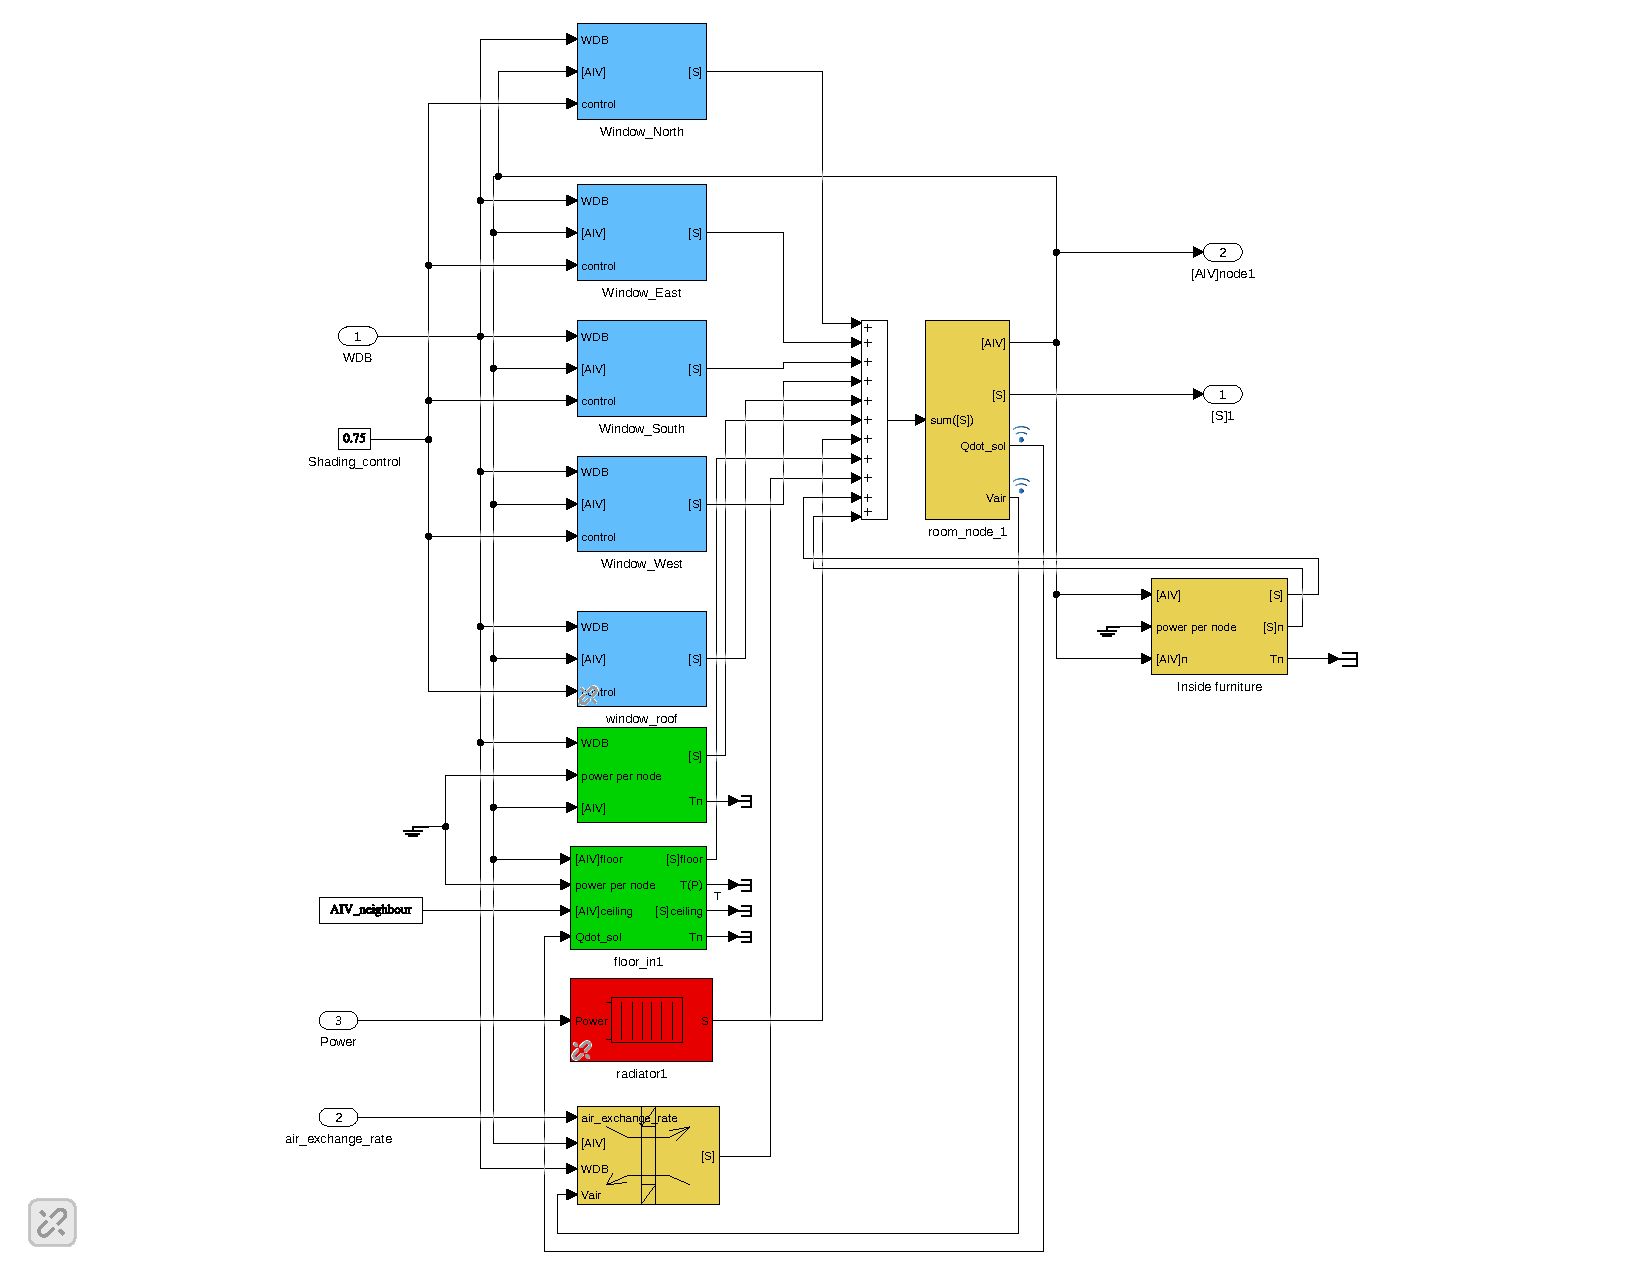
\includegraphics[width = \textwidth]{Images/polydome_room_model.pdf}
    \caption{Simulink Schema of the CARNOT \pdome\ building model}
    \label{fig:CARNOT_polydome}
\end{figure}

\clearpage

Finally, the  Simulink model is completed by adding a \textit{Weather Data File}
containing weather measurements for a whole year, and a \textit{Weather
Prediction} block responsible for sending weather predictions to the MPC.\@ The
controller itself is defined in Python and is connected to Simulink via three
TCP/IP sockets. Details on the implementation are presented in
Section~\ref{sec:implementation}.

\subsection{Physical dimensions}\label{sec:Physical_dimensions}

The \pdome\ building is a dome-shaped, single-zone building serving the role
of classroom for audiences of around one hundred students.

Most of the necessary measurements are already available from the
\citetitle*{nattererPolydomeTimberShell1993} article by
\textcite{nattererPolydomeTimberShell1993}. It presents the \pdome\ geometry as
having a floor area of 25m $\times$ 25m, a maximum height of the building of 7m,
walls of a maximum height of 3m. The roof is a spherical cap with a radius of
approximately 28m.

One particularity of the \pdome\  is the presence of four large skylights on the
roof. An estimate of their size has been made using images from \textit{Google
Maps Satellite View}~\cite{GoogleMaps}, with the included measurement tool. These
measurements are presented in Figure~\ref{fig:Google_Maps_Skylights}. The
skylights are measured to be squares of edge 2.5m.

\begin{figure}[ht]
    \centering
    \vspace{-10pt}
    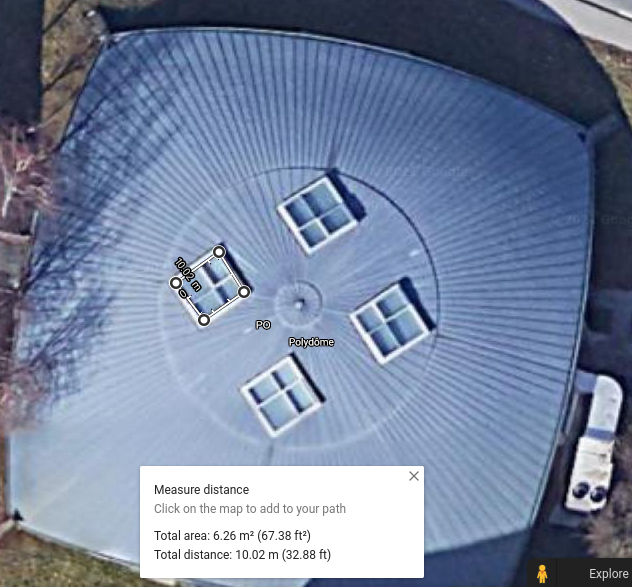
\includegraphics[width = 0.75\textwidth]{Images/google_maps_polydome_skylights}
    \caption{Google Maps Satellite view of the \pdome\ building}
    \label{fig:Google_Maps_Skylights}
\end{figure}

The only remaining missing piece of information is the \textit{stem wall}
height, which is the height of the walls from the ground on which the dome
ceiling directly resides. Due to the limited campus access, this measure has
also been approximated from a Google Maps image, presented in
Figure~\ref{fig:Google_Maps_Streetview}. An object of known size has been used
as reference, after which the following measurements have been done in
\citetitle{kimballGIMPGNUImage}~\cite{kimballGIMPGNUImage} using the
\textit{Measure Tool}.

The chosen reference object is the \pdome\ \acrshort{hvac} system, the full
description of which is presented in Section~\ref{sec:HVAC_parameters}, and
which has a known height of 2061mm \cite{aermecRoofTopManuelSelection}.

\clearpage

\begin{figure}[ht]
    \centering
    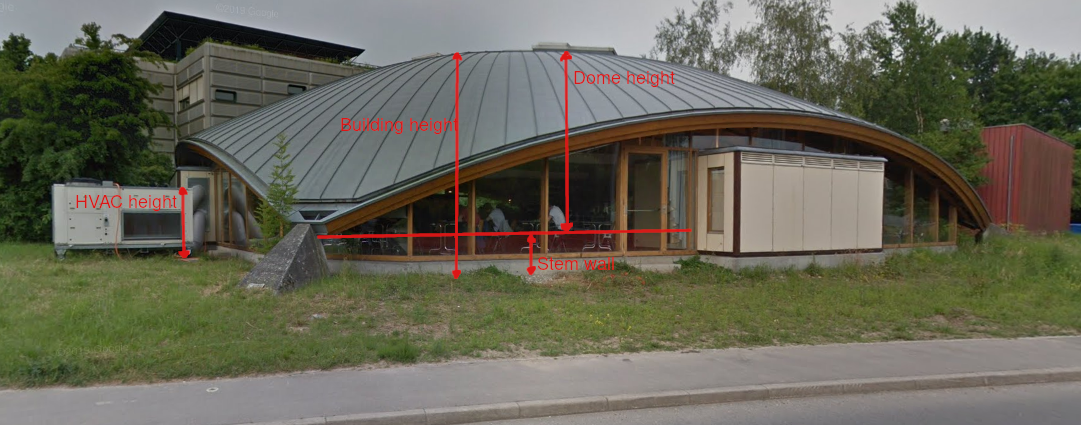
\includegraphics[width = \textwidth]{Images/polydome_streetview_annotated}
    \caption{Google Maps StreetView view of the \pdome\ building}
    \label{fig:Google_Maps_Streetview}
\end{figure}

The graphical analysis resulted in the measurements presented in
Table~\ref{tab:GIMP_measurements}:

\begin{table}[ht]
%\vspace{-8pt}
\centering
    \begin{tabular}{||c c c c||}
        \hline
        Object & Size [px] & Size[mm] & Size[m]\\
        \hline \hline
        \acrshort{hvac} height & 70 & 2100 & 2.1 \\
        Building height & 230 & 6900 & 6.9 \\
        Stem wall & 45 & 1350 & 1.35 \\
        Dome height & 185 & 5550 & 5.55 \\
        \hline
    \end{tabular}
\caption{Calculated Dome Dimensions}
\label{tab:GIMP_measurements}
\end{table}

For a validation of the results shown in Figure~\ref{tab:GIMP_measurements} it
is possible to compare the total \pdome\ building height measured in GIMP with
the value presented beforehand. The graphical measure of 6.9m is indeed very
close to the described height of 7m.

These measurements can be used to set the size parameters of all the nodes in
the model:

\begin{itemize}
    \item Side windows with a size of 2m $\times$ 25m each
    \item Roof window with a size of 5m $\times$ 5m, cumulative surface of all
        the skylights
    \item Ceiling with a size of 25m $\times$ 25m
    \item Floor with a size of 25m $\times$ 25m
\end{itemize}

\subsection{Internal volume}

The \pdome\ building has a structure that is mostly based on a dome shape, with
the difference that the dome portion of the building does not reach the ground,
but stands above it at a height of approximately $1.35$m (cf.
Table~\ref{tab:GIMP_measurements}), with the large side windows extending to the
ground and creating a \textit{stem wall} for the dome to sit on.

The total internal volume of the \pdome\ building can therefore be approximated
by computing the sum volumes of the two elements: the stem and the dome.

Geometrically, a dome is a portion of a sphere cut off by a plane. Its volume
can therefore be computed in a similar fashion to that of a complete sphere.

A sphere can be regarded as volume of rotation of function $f(x)$ (cf.
Equation~\ref{eq:rot_func}) around the x axis, where $R$ is the sphere radius
and $x \in [0, 2r]$: 

\begin{equation}\label{eq:rot_func}
    f(x) = \sqrt{R^2 - (x-R)^2} = \sqrt{2Rx - x^2}
\end{equation}

It is therefore possible to compute the volume of a dome by integrating $f(x)$
up to the dome height $h$, as presented in Equation~\ref{eq:rot_vol}. 

\begin{equation}\label{eq:rot_vol}
    \begin{aligned}
        V &= \pi \int_0^h f(x)^2 dx \\
          &= \pi \int_0^h (2Rx - x^2)dx \\
          &= \pi \left( Rx^2 - \frac{1}{3}x^3 \right)_0^h \\
          &= \frac{\pi h^2}{3} (3R - h) \\
    \end{aligned}
\end{equation}

The volume of the \pdome\ dome is computed  by first finding the radius of the
complete sphere, the radius of curvature (cf.
Equation~\ref{eq:radius_curvature}, where $h$ is the height of the dome and $r$
is the radius of the base of the dome) and plugging it in
Equation~\ref{eq:rot_vol}.

\begin{equation}\label{eq:radius_curvature}
    R_c = \frac{r^2 + h^2}{2h}
\end{equation}

The volume of the dome is then given by: 

\begin{equation}
    V_d = \frac{1}{3} \pi h^2 (3R_c - h) = \frac{1}{6} \pi h (3r^2 + h^2)
\end{equation}

The stem of the \pdome\ is approximated to a cube of edge 25m, and its volume can
therefore be calculated as: 

\begin{equation}
    V_s = l_s^2 \times h_s
\end{equation}

The total volume of the building is then given as: 

\begin{equation}
    V = V_d + V_s = \frac{1}{6} \pi h (3r^2 + h^2) + l_s^2 \times h_s
\end{equation}

Numerically, considering a dome diameter of 28m, a dome height of 5.55m and a stem
wall edge of 25m, we get the approximate volume of the building:
\begin{equation}\label{eq:numerical_volume}
    V = V_d + V_s = 1798.22m^3 + 843.75m^3 = 2641.97m^3 \approx 2650m^3
\end{equation}

The value presented in Equation~\ref{eq:numerical_volume} is used directly in
the \textit{room\_node} element of the CARNOT model (cf.
Figure~\ref{fig:CARNOT_polydome}), as well as the calculation of the Air
Exchange Rate, presented in Section~\ref{sec:Air_Exchange_Rate}.

\subsection{Furniture}

The main function of the \pdome\ building is serving as a classroom for around
one hundred students. It has wood furniture consisting of chairs and tables, as
well as a wooden stage in the center of the building, meant to be used for
presentations. The building also contains a smaller room, housing all the
necessary technical equipment (cf. Figure~\ref{fig:Google_Maps_Streetview}).

The most accurate way of including information on the furniture in the CARNOT
model would be to manually compute the mass, volume and materials for each of
the chairs, tables, etc.\ but due to the restricted access to the building a
simpler approximation has been made.

\textcite{johraNumericalAnalysisImpact2017} present a methodology to model the
furniture in buildings for different materials, as well as an \textit{equivalent
indoor content material} that is meant to approximate the furniture content of
an office building. These values for mass content, surface area, material
density and thermal conductivity have been taken as the basis for the \pdome\
furniture content approximation, with the assumption that, since the \pdome\ is
still mostly empty, it has approximately a quarter of the furniture present in a
fully furnished office.

The full set of furniture is, therefore, approximated in the CARNOT model as a
wall, with the numerical values for mass, surface, thickness and volume
presented below.

\subsubsection*{Surface}
% surface:
% 1/4 * 1.8 [m2/m2 of floor space] * 625 m2 surface = 140 m2
% 140 m2 = [7 20] m [height width]

The equivalent material is taken to have a surface of 1.8 $\text{m}^2$ per each
$\text{m}^2$ of floor area~\cite{johraNumericalAnalysisImpact2017}. With a floor
area of 625 $\text{m}^2$, and assuming the furnishing of the building is a
quarter that of a fully-furnished office, the \pdome\ furniture equivalent wall
has a surface area of:

\begin{equation}
    S_f = \frac{1}{4} \cdot 1.8 \left[\frac{\text{m}^2}{\text{m}^2}\right]
    \cdot 625\ \left[\text{m}^2\right] = 281.25 \left[\text{m}^2\right]
\end{equation}

Since a wall has two large faces, the total surface gets divided between them
for a surface of each face of: 

\begin{equation}
    S_{f, \text{face}} = 
    \frac{1}{2} \times S_f \approx 140 \left[\text{m}^2\right]
\end{equation}

\subsubsection*{Mass}
% mass:
% 1/4 * 40 [kg/m2 of floor space] * 625 m2 surface = 6250 kg

The mass of the furniture equivalent wall is computed using the same
methodology, considering 40 kg of furniture mass per $\text{m}^2$ of floor
surface.

\begin{equation}
    M_f = \frac{1}{4} \cdot 40 \cdot 625\ \left[\text{m}^2\right] = 6250\
    \left[\text{m}^2\right]
\end{equation}

\subsubsection*{Volume}
% volume:
% 6250[kg]/600[kg/m3] = 10.41 [m3]

The volume of the furniture equivalent wall is calculated with the help of the
equivalent mass and densities:

\begin{equation}
    V_f = \frac{M_f}{\rho_f} = \frac{6250}{600}
    \left[\frac{\text{kg}}{\text{kg}/\text{m}^3}\right]
    = 10.41\ \left[\text{m}^3\right]
\end{equation}

\subsubsection*{Thickness}
% thickness:
%10.41[m3]/140[m2] = 0.075m = 7.5cm

The last parameter of the furniture equivalent wall is computed by dividing its
volume by the surface:

\begin{equation}
    h_f = \frac{V_f}{S_{f, \text{face}}} 
    = \frac{10.41}{140} \left[\frac{m^3}{m^2}\right]
    = 0.075\ \left[\text{m}\right] = 7.5\ \left[\text{cm}\right]
\end{equation}


\subsection{Material properties}

In order to better simulate the behaviour of the real \pdome\ building, it is
necessary to approximate the building materials and their properties as close as
possible. This section goes into details and arguments for the choice of
parameters for each of the CARNOT nodes' properties.

\subsubsection{Windows}

The windows are made of two glass panes of thickness 4mm each.

The values of the heat transfer coefficient (U-factor) can vary greatly for
different window technologies, but an educated guess can be made on the lower
and upper bounds based on the age and location of the building. 

Window manufacturers state
the U-factor for double glass windows to be between 2.8 \(\frac{W}{m^2K}\) for
older manufacturing techniques and 1.2 \(\frac{W}{m^2K}\) for newer
models~\cite{WhatAreTypical2018}. 

The US Energy Department states that the
typical U-factor values for modern window installations is in the range of 0.2
--- 1.2 \(\frac{W}{m^2K}\)~\cite{GuideEnergyEfficientWindows}. 

The European flat glass association claims that the maximum allowable U-factor
value for new window installations in the private sector buildings in
Switzerland is 1.5
\(\frac{W}{m^2K}\)~\cite{glassforeuropeMinimumPerformanceRequirements2018}.

Considering the aforementioned values, and the fact the \pdome\ building was
built in 1993~\cite{nattererModelingMultilayerBeam2008}, the default U-factor of
1.8 \(\frac{W}{m^2K}\) has been deemed appropriate.

The total solar energy transmittance $[g]$ and transmittance in the visible
range $[v_g]$ can vary in the range of 0.1 --- 0.9 depending on manufacturing
technology, tint, etc. The average values of 0.7 and 0.65 respectively have been
chosen for this case.

The values for glass density and heat capacity have been left at their default
values of 2500 \(\frac{kg}{m^3}\) and 1008 \(\frac{J}{kgK}\) respectively.

\subsubsection{Roof and Floor}

%%% Roof
% [5cm wood, 10cm insulation, 5cm wood]
% Conductivity for each material
% Heat capacity for each material
% Density for each material

The roof structure has been assumed to be made out of 10 cm of insulation,
enclosed on each side by 5 cm of wood.

%%% Floor
% [5cm wood, 10cm insulation, 20cm concrete]
% Conductivity for each material
% Heat capacity for each material
% Density for each material

The floor composition has been taken as consisting of, from top to bottom, 5 cm
wood, 10 cm insulation followed by 20 cm of concrete. 

All the necessary values to characterise these materials have been taken
from~\cite{BuildingsHeatTransferData} and are presented in
Table~\ref{tab:material_properties}: 

\begin{table}[ht]
%\vspace{-8pt}
\centering
    \begin{tabular}{||c c c c||}
        \hline
        Material & Thermal Conductivity $k$ $[\frac{W}{mK}]$ & Specific Heat
        Capacity $c$ $[\frac{J}{kgK}]$ & Density $\rho$ $[\frac{kg}{m^3}]$
        \\
        \hline \hline
        Plywood & 0.12 & 1210 & 540 \\
        Insulation & 0.03 & 1200 & 40 \\
        Concrete & 1.0 & 700 & 2500 \\
        \hline
    \end{tabular}
    \caption{Material properties for roof and floor elements}
\label{tab:material_properties}
\end{table}

\subsection{HVAC parameters}\label{sec:HVAC_parameters}

The \pdome\ is equipped with an \textit{AERMEC RTY-04} \acrshort{hvac} system.
According to the manufacturer's manual~\cite{aermecRoofTopManuelSelection}, this
\acrshort{hvac} houses two compressors of power 11.2 kW and 8.4 kW respectively,
an external ventilator of power 1.67 kW, and a reflow ventilator of power 2 kW.
The unit has a typical \acrlong{eer} (\acrshort{eer}, cooling efficiency) of 4.9
--- 5.1 and a \acrlong{cop} (\acrshort{cop}, heating efficiency) of 5.0, for a
maximum cooling capacity of 64.2 kW. 

One particularity of this \acrshort{hvac} unit is that during summer, only one
of the two compressors are running. This results in a higher \acrlong{eer}, in
the cases where the full cooling capacity is not required.

\subsubsection*{Ventilation}

According to the manufacturer manual \cite{aermecRoofTopManuelSelection}, the
\acrshort{hvac} unit's external fan has an air flow ranging between 4900
$\text{m}^3/\text{h}$ and 7000 $\text{m}^3/\text{h}$.

\subsubsection*{Air Exchange Rate}\label{sec:Air_Exchange_Rate}

The air exchange rate, also known as `air changes per hour', represents the
number of times the air in a room gets replaced with new air. It can be
computed by dividing the air flow through the room by the room volume:

\begin{equation}
    \text{Air exchange rate} = \frac{\text{Air flow}}{\text{Total volume}}
\end{equation}

In the case of the \pdome\ and its \acrshort{hvac}, this results in an airflow
range of:

\begin{equation}
    \begin{aligned}
        \text{Air exchange rate} &= \frac{4900}{2650} 
        - \frac{7000}{2650} &\left[\frac{\text{m}^3/\text{h}}{\text{m}^3}\right]\\
                            &= 1.85 - 2.64 &\left[\frac{1}{\text{h}}\right]
    \end{aligned}
\end{equation}

As it will be shown in Section~\ref{sec:CARNOT_experimental}, the external fan
is continuously running. The \textit{Air exchange rate} has therefore been fixed
to a value of 2.5 for the duration of the whole simulation. The real airflow
could, of course, vary depending on a multitude of external factors, but they
would require more precise measurements to estimate.

\subsection{Validating against experimental data}\label{sec:CARNOT_experimental}

In order to confirm the validity of the model, it is necessary to compare the
CARNOT models' behaviour against that of the real \pdome\ building.

Section~\ref{sec:CARNOT_expdata} presents the available experimental data,
Section~\ref{sec:CARNOT_WDB} details the transformation of the available data
into CARNOT's WDB format, and Section~\ref{sec:CARNOT_comparison} details a
qualitative analysis of the differences.

\subsubsection{The available experimental data}\label{sec:CARNOT_expdata}

All the experimental data used for the validation of the CARNOT model has been
collected previously for another
study~\cite{fabiettiMultitimeScaleCoordination2018}, where it has been used to
identify a State Space model for the \pdome\ building.

The data has been collected in the time span of June to August 2017, and is
divided in seven different experiments, as presented in
Figure~\ref{tab:exp_dates}. The available measurements are the \textit{Outside
Temperature}, \textit{Solar Irradiation}, \textit{Electrical power consumption}
of the \acrshort{hvac}, and two measurements of \textit{Inside Temperature} in
different parts of the room.

\begin{table}[ht]
\centering
    \begin{tabular}{||c c c||}
        \hline
        Exp no. & Start Date & End Date\\
        \hline \hline
        1 & 01.06.2017 20:00 & 03.06.2017 17:00 \\
        2 & 10.06.2017 16:00 & 12.06.2017 06:00 \\
        3 & 16.06.2017 20:00 & 19.06.2017 06:00 \\
        4 & 19.06.2017 20:00 & 22.06.2017 06:00 \\
        5 & 30.06.2017 20:00 & 03.07.2017 06:00 \\
        6 & 07.07.2017 20:00 & 10.06.2017 06:00 \\
        7 & 13.06.2017 20:00 & 20.06.2017 06:00 \\
        \hline
    \end{tabular}
\caption{\pdome\ experimental measurements}
\label{tab:exp_dates}
\end{table}

\clearpage

As mentioned previously, the external fan of the \acrshort{hvac} is constantly
running.  This can be seen in Figure~\ref{fig:Polydome_electricity} as the
electricity consumption of the \acrshort{hvac} has a baseline of 1.67 kW.

\begin{figure}[ht]
    \centering
    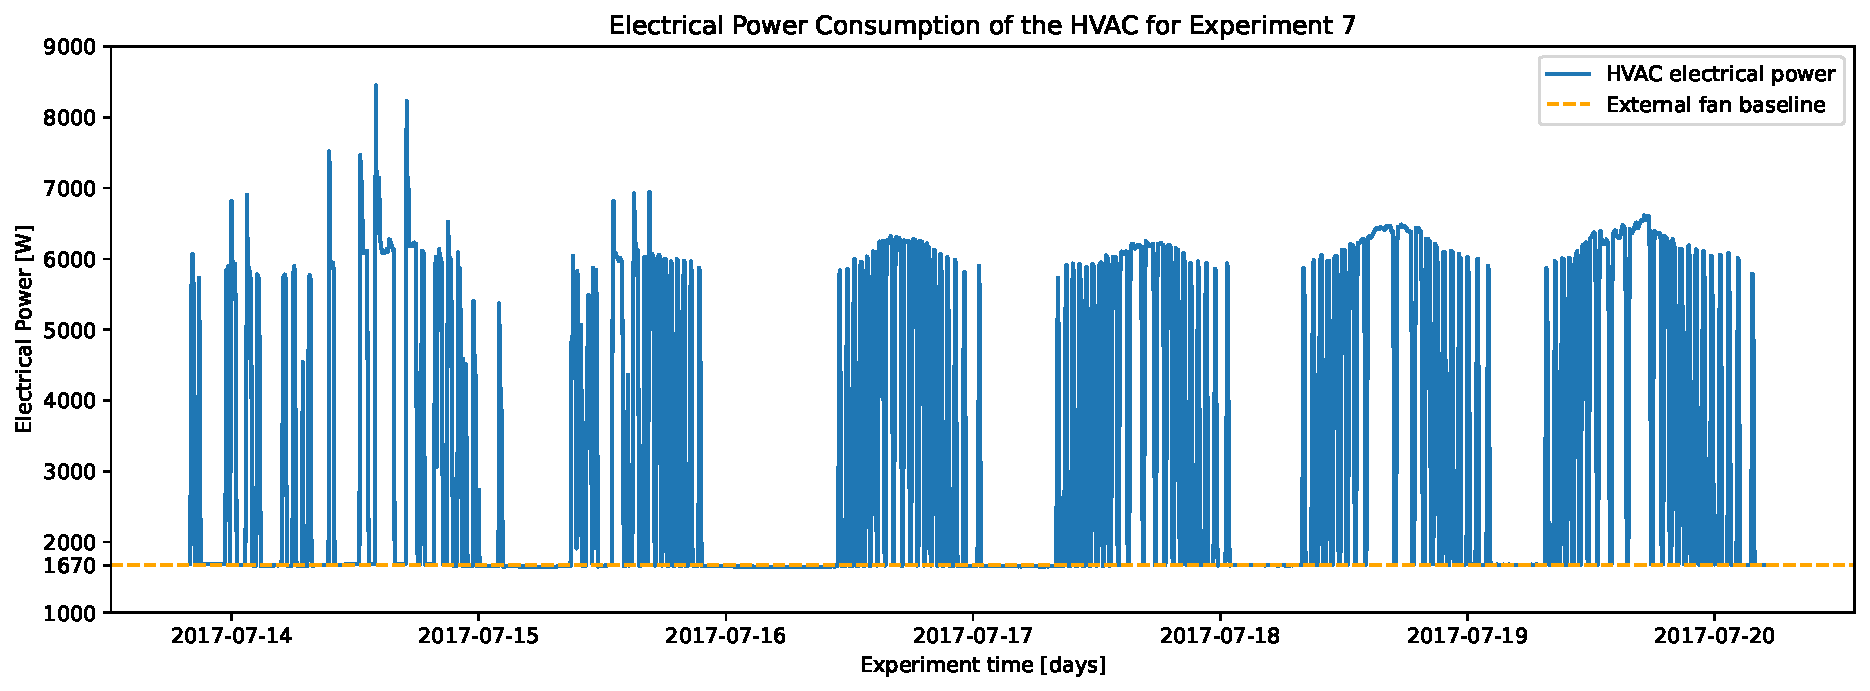
\includegraphics[width = \textwidth]{Plots/Fan_baseline.pdf}
    \caption{Electrical Power consumption of the \pdome\ \acrshort{hvac} for Experiment 7}
    \label{fig:Polydome_electricity}
\end{figure}

Figure~\ref{fig:Polydome_electricity} also gives an insight into the workings of
the \acrshort{hvac} when it comes to the combination of the two available
compressors. The instruction manual of the
\acrshort{hvac}~\cite{aermecRoofTopManuelSelection} notes that in summer only
one of the compressors is running. This allows for a larger \acrshort{eer} value
and thus better performance. We can see that this is the case for most of the
experiment, where the power consumption caps at around 6~kW, which is the
maximum power consumption of one compressor. There are, however, moments during
the first part of the experiment where the power momentarily peaks over the 6~kW
limit, and goes as high as around 9~kW. This most probably happens when the
\acrshort{hvac} decides that the difference between the set point temperature
and the actual measured values is too large to compensate with a single
compressor.

Figure~\ref{fig:Polydome_exp7_settemp} presents the values of the set point
temperature and the measured internal temperature. 

\begin{figure}[ht]
    \centering
    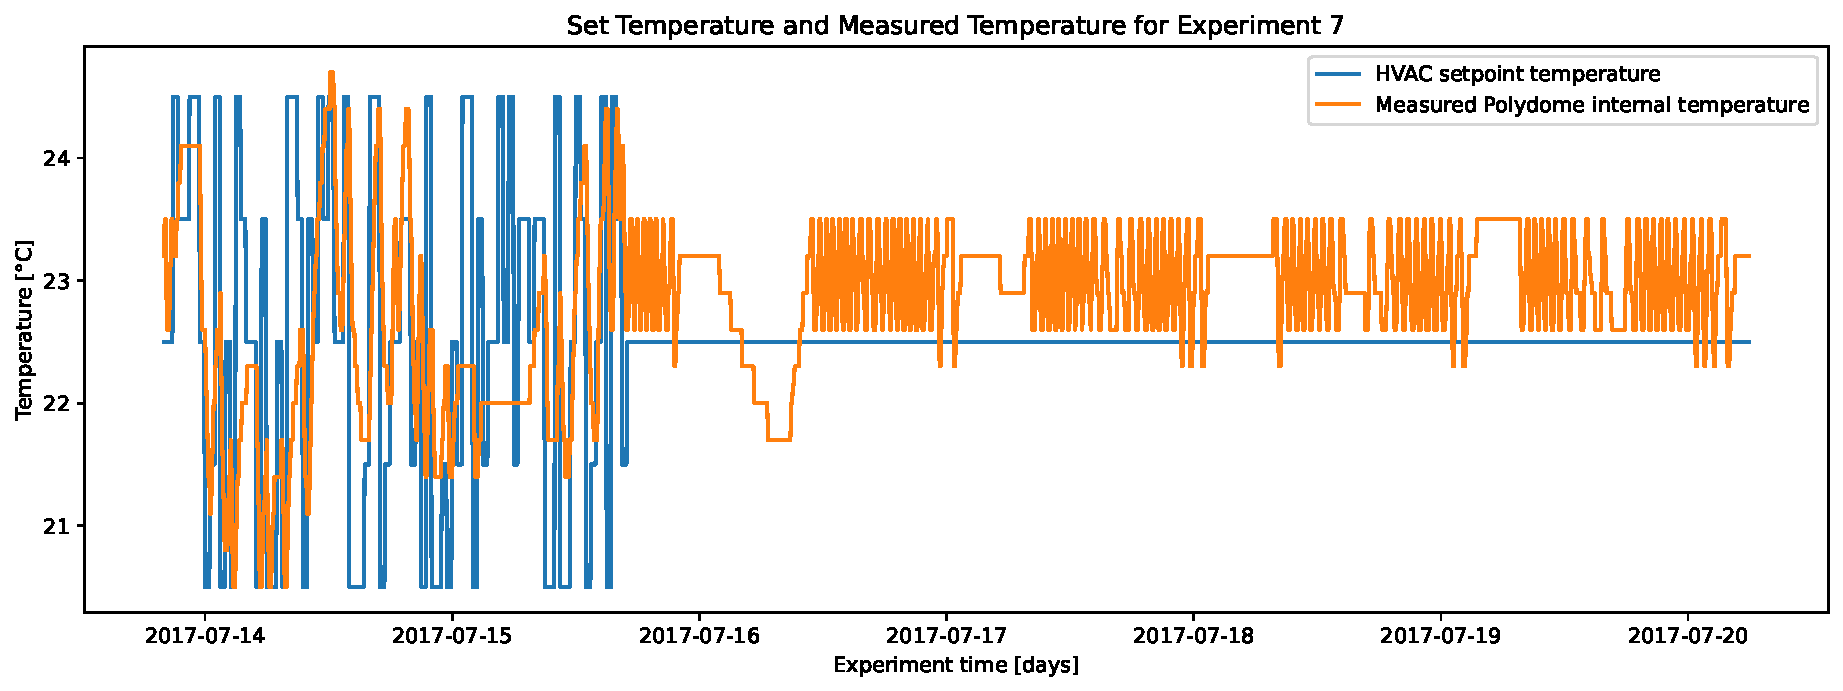
\includegraphics[width = \textwidth]{Plots/Exp_settemp.pdf}
    \caption{Measured vs set point temperature of the \acrshort{hvac} for Experiment 7}
    \label{fig:Polydome_exp7_settemp}
\end{figure}

A few observations can be made on these measurements. First, the second
compressor is indeed turned on during the first part of the experiment, when the
set point differs greatly from the measured temperature. Second, for the
beginning of Experiment 7, as well as the majority of the other experiments, the
set point temperature is the value that gets changed in order to excite the
system, and since the \acrshort{hvac}'s controller is on during identification,
it will oscillate between using one or two compressors. Lastly, it is possible
to notice that the \acrshort{hvac} is not turned on during the night, with the
exception of the external fan, which continues running.

\subsubsection{The CARNOT WDB weather data format}\label{sec:CARNOT_WDB}

For a correct simulation of the building behaviour, CARNOT requires not only the
detailed definition of the building blocks/nodes, but also a very detailed set
of data on the weather conditions. This set includes detailed information on the
sun's position throughout the simulation (zenith and azimuth angles), the
\acrfull{dhi} and \acrfull{dni}, direct and diffuse solar radiation on surface,
as well as information on the ambient temperature, humidity, precipitation,
pressure, wind speed and direction, etc.  A detailed overview of each
measurement necessary for a simulation is given in the CARNOT user
manual~\cite{CARNOTManual}.

In order to compare the CARNOT model's performance to that of the real \pdome,
it is necessary to simulate the CARNOT model under the same set of conditions as
the ones present during the experimental data collection. In order to do this,
all the missing values that are required by the simulation have to be filled. In
some cases, such as the sun angles it is possible to compute the exact values,
but in other cases the real data is not available, which means that it has to be
inferred from the available data.

The information on the zenith and azimuth solar angles can be computed exactly
if the position and elevation of the building are known. The GPS coordinates and
elevation information is found using a map~\cite{ElevationFinder}. With that
information available, the zenith, azimuth angles, as well as the \acrfull{aoi}
are computed using the Python pvlib
library~\cite{f.holmgrenPvlibPythonPython2018}.

As opposed to the solar angles, which can be computed exactly from the available
information, the Solar Radiation Components (DHI and DNI) have to be estimated
from the available measurements of GHI, zenith angles (Z) and datetime
information.  \textcite{erbsEstimationDiffuseRadiation1982} present an empirical
relationship between GHI and the diffuse fraction DF and the ratio of GHI to
extraterrestrial irradiance $K_t$, known as the Erbs model. The DF is then used
to compute DHI and DNI as follows:

\begin{equation}
    \begin{aligned}
        \text{DHI} &= \text{DF} \times \text{GHI} \\
        \text{DNI} &= \frac{\text{GHI} - \text{DHI}}{\cos{\text{Z}}}
    \end{aligned}
\end{equation}

All the other parameters related to solar irradiance, such as the in-plane
irradiance components, in-plane diffuse irradiance from the sky and the ground
are computed using the Python pvlib.

The values that can be neither calculated nor approximated from the available
data, such as the precipitation, wind direction, incidence angles in place of
vertical and main/secondary surface axis, have been replaced with the default
CARNOT placeholder value of -9999. The relative humidity, cloud index, pressure
and wind speed have been fixed to the default CARNOT values of 50\%, 0.5, 96300
Pa, 0 $\text{m}/\text{s}$ respectively.

\subsubsection{\pdome\ and CARNOT model comparison}\label{sec:CARNOT_comparison}

With the \acrshort{wdb} data compiled, we can now turn to simulating the CARNOT
model and compare its behaviour to that of the real \pdome\ building. 

Unfortunately, one crucial piece of information is still missing: the amount of
heat that the \acrshort{hvac} either pumps in or takes out of the building at
any point in time.  This value could be approximated from the information of
electrical power consumption and the \acrshort{eer}/\acrshort{cop} values given
that it is known if the \acrshort{hvac} is in either heating or cooling mode. 

This information lacking in the existing experimental datasets, the heat
supplied/ taken out of the system has been inferred from the electrical energy
use, measured building temperature and \acrshort{hvac} temperature set point,
with the assumption that the \acrshort{hvac} is in cooling mode whenever the
measurements are higher than the set point temperature, and is in heating mode
otherwise. As it can already be seen in Figure~\ref{fig:Polydome_exp7_settemp},
this is a very strong assumption, that is not necessarily always correct. It
works well when the measurements are very different from the set point, as is
the case in the first part of the experiment, but this assumption is false for
the second part of the experiment, where the set point temperature remains fixed
and it is purely the \acrshort{hvac}'s job to regulate the temperature.

\begin{figure}[ht]
    \centering
    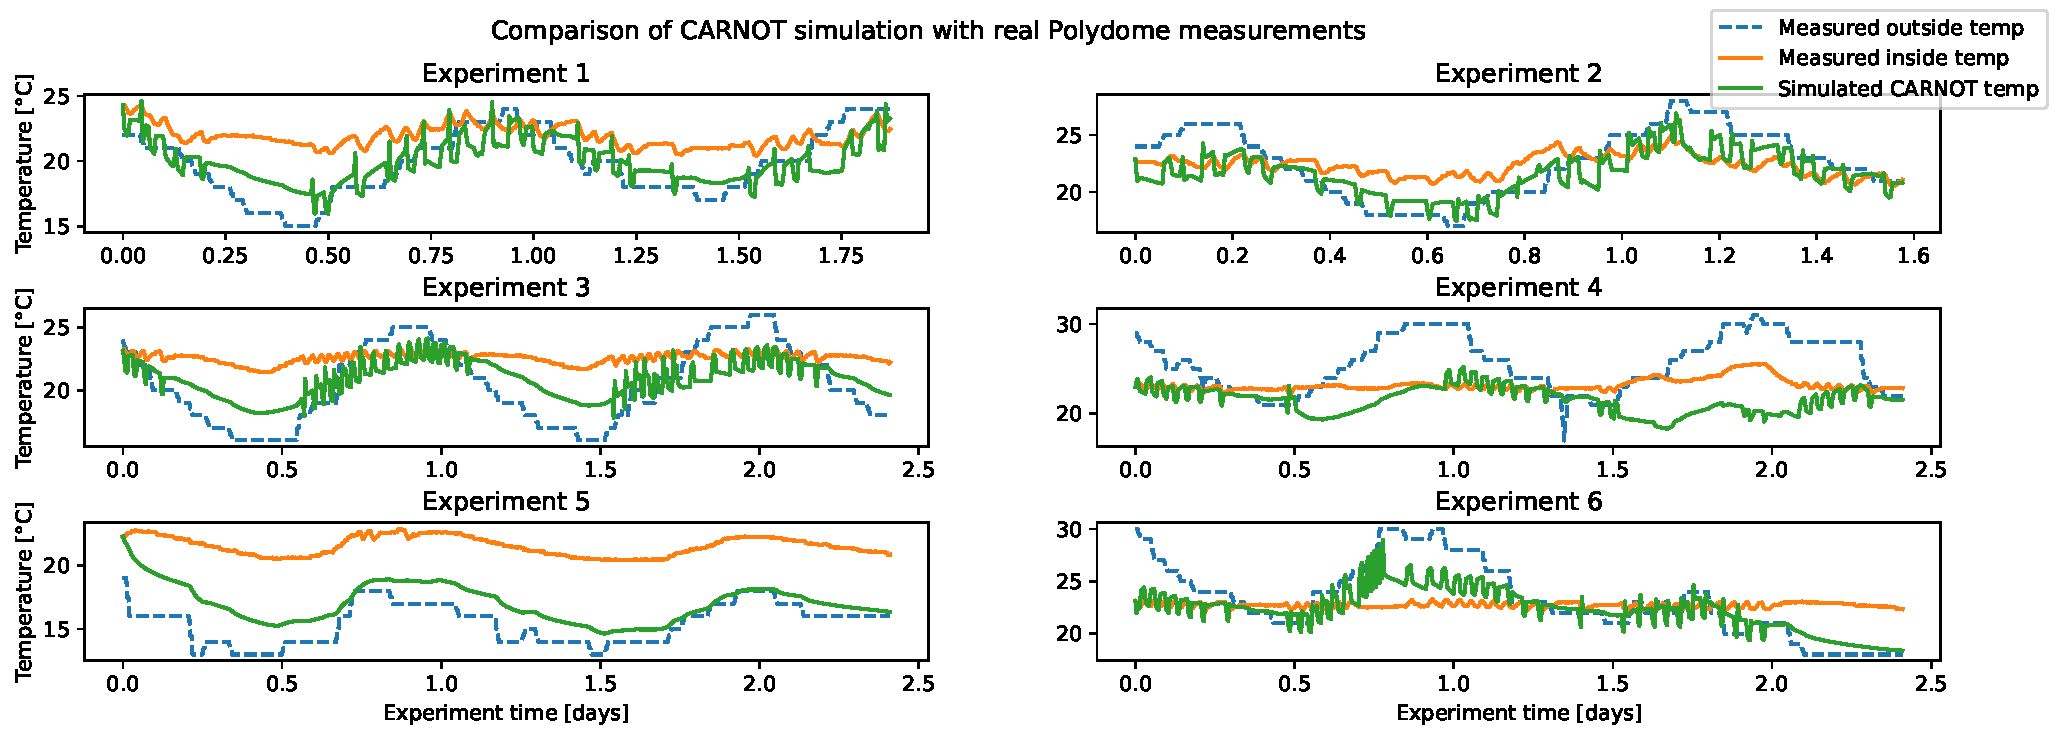
\includegraphics[width = \textwidth]{Plots/CARNOT_comparison_1.pdf}
    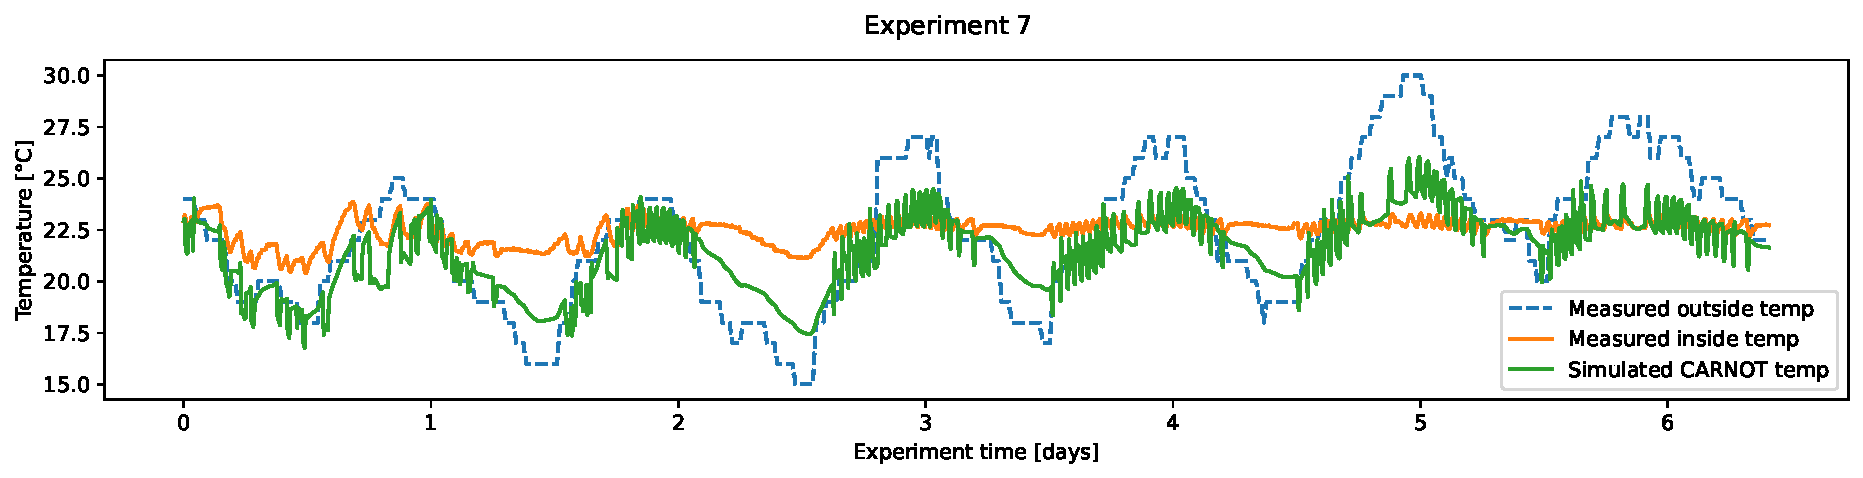
\includegraphics[width = \textwidth]{Plots/CARNOT_comparison_2.pdf}
    \caption{Measured vs CARNOT simulated temperature for the Experimental
    Datasets}
    \label{fig:CARNOT_simulation_validation}
\end{figure}

The results of the seven simulations are presented in
Figure~\ref{fig:CARNOT_simulation_validation}. Overall, the simulated
temperature has the same behaviour as the real \pdome\ measurements. A more
detailed inspection shows that for most of the experiments, the simulated
temperature is much more volatile than the true measurements. This could be due
to an overestimated value of the Air Exchange Rate, underestimated amount of
furniture in the building or, more probably, miscalculation of the
\acrshort{hvac}'s heating/cooling mode. Of note is the large difference in
behaviour for the Experiments 5 and 6. In fact, for these experiments, the
values for the electrical power consumption greatly differ in shape from the
ones presented in the other datasets, which could potentially mean erroneous
measurements, or some other underlying problem with the data.

Finally, it is possible to conclude that the CARNOT building behaves comparably
to the real \pdome\, even if not perfectly simulates its behaviour. These
differences  could come from multiple factors --- missing information that had
to be inferred and/or approximated, such as the Air Exchange Ratio, the heat
provided/extracted, the amount of furniture in the building, the overall shape
and size of the building, as well as possibly errors in the experimental data
used for validation. A more detailed analysis of the building parameters would
have to be done in order to find the reasons and eliminate these discrepancies.

\clearpage
